%!TEX root = ../pres.tex

\begin{frame}
	\frametitle{Behavioral Cloning}
	\onslide<1->{\begin{center}
		\textbf{Behavioral Cloning:} Supervised learning in MDPs using and expert agent expert $\pi^*$!
	\end{center}}
	\onslide<2->{Given expert examples $\scriptd = (s_t, a_t = \pi^*(s_t))$ and a model $\pi_\theta$ find $\theta^*$ st
	\begin{equation*}
		\theta^*  = \argmin_\theta \scriptl(a_t, \pi_\theta(s_t)).
	\end{equation*}
	where $\scriptl$ is some loss function.}
	\begin{itemize}
		\item<3->  Show, don't tell! 
		\item<4-> No complicated machinery, just standard ML.
	\end{itemize}
\end{frame}


\begin{frame}
	\frametitle{Behavioral Cloning}
		\textbf{Issue: Compounding Error}
		\begin{columns}
			\begin{column}{0.5\textwidth}
			Given some irreducible error $\epsilon =0.001$
				\begin{itemize}
					\item $\scriptl(a_0, \pi_\theta(s_0)) = \epsilon$
					\item $\scriptl(a_1, \pi_\theta(s_1)) = 2\epsilon$
					\item $\scriptl(a_2, \pi_\theta(s_2)) = 3\epsilon$
					\item $\scriptl(a_3, \pi_\theta(s_3)) = 4\epsilon$
					\item $\scriptl(a_4, \pi_\theta(s_4)) = 5\epsilon$
				\end{itemize}
			\end{column}
			\begin{column}{0.5\textwidth}
				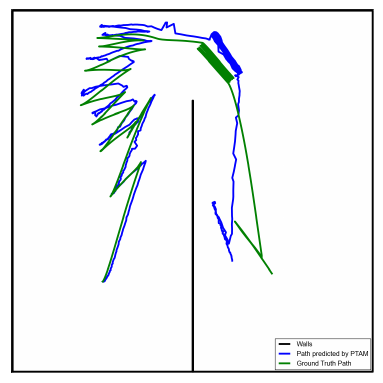
\includegraphics[width=0.99\textwidth]{bh1.png}
			\end{column}
		\end{columns}
\end{frame}

\begin{frame}
	\frametitle{Behavioral Cloning}
		\begin{columns}
			\begin{column}{0.6\textwidth}
			\onslide<1->{
			\textbf{Issue: Distribution Mismatch}
			\begin{itemize}
				\item States expert dataset $\scriptd$ generated by $\pi^*$ have
				different distribution than those generated by $\pi_\theta$. 

				{$\implies$ No self correction.}
			\end{itemize}
			}

			\onslide<2->{\textbf{Solution: DAgger}.
			\begin{itemize}
				\item Do BC on $\scriptd$ and generate $E_0$ states generated by $\pi_\theta.$
				\item Label $E_0$ with expert level actions and add to $\scriptd$.
			\end{itemize}
			}
			\end{column}
			\begin{column}{0.4\textwidth}
				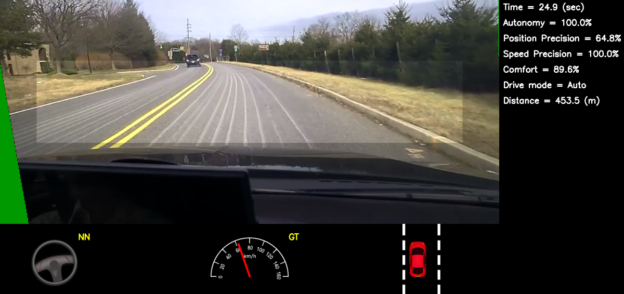
\includegraphics[width=0.99\textwidth]{bh2.png} \\
				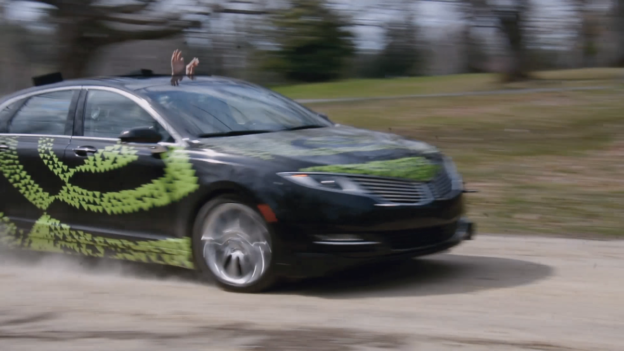
\includegraphics[width=0.99\textwidth]{bh3.png}
			\end{column}
		\end{columns}
\end{frame}